
\chapter{基础知识}

\section{晶体结构}
固体是处于凝固状态下的物体,通常具有一定的质量和体积。
按照其内部原子的排列情况可分为三种主要的结构类型,即\textbf{单晶、多晶和非晶}。
\begin{itemize}
    \item \textbf{单晶}:长程有序(整体有序,宏观尺度,通常包含整块晶体材料,一般在毫米量级以上);
    \item \textbf{多晶}:长程无序,短程有序(团体有序,成百上千个原子的尺度,每个晶粒的尺寸通常在微米量级);
    \item \textbf{非晶}:基本无序(局部、个体有序,几个原子或分子尺度,纳米级)
\end{itemize}

\begin{figure}[hbt]
  \centering
  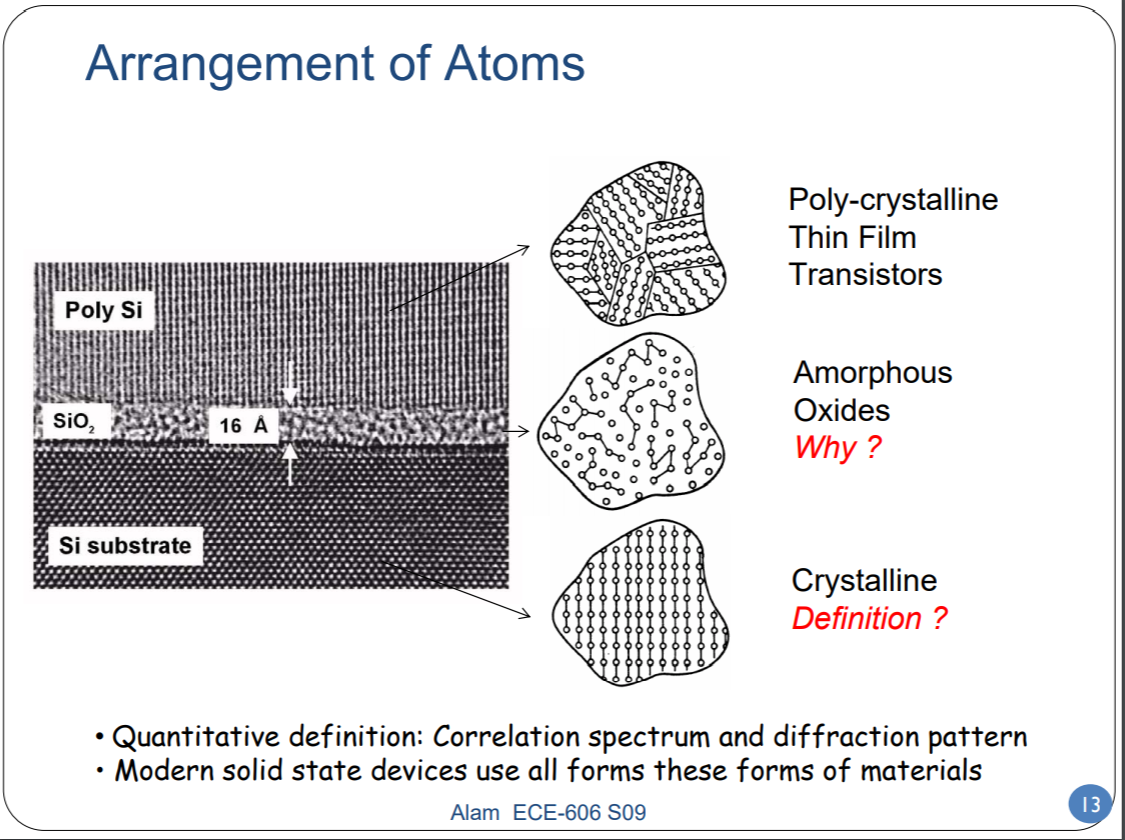
\includegraphics[width = .8\linewidth ]{chapter1/crystals.png}
  \caption{现代固态器件上拥有所有晶体形态}
  \label{fig-crystals}
\end{figure}

图\ref{fig-crystals}展示了三种晶体的结构示意图,在现代半导体器件工艺中,通常三种晶体都会被用到,如图中多晶硅栅极、非晶氧化绝缘层和单晶硅衬底。
通常若不特别说明,晶体特指单晶。

\subsection{原胞与晶胞}
晶体在几何空间上,有着很强的周期性。
为了描述这种特殊的原子排列,引入\textbf{格点}可以更好的分析,同时与之相关的概念还有\textbf{晶格}、\textbf{晶胞}和\textbf{原胞}。其示意图见图\ref{fig-lattice}和图\ref{fig-vector}。
\begin{itemize}
    \item \textbf{晶格(Lattice)}:晶体中原子的周期性排列情况,分为简单晶格\footnote{Cu, Fe, Ag}和复式晶格\footnote{NaCl}两大类。
    \item \textbf{格点(Lattice Point)}:晶格中用来表示原子阵列的点。
    \item \textbf{晶胞(Unit Cell)}:也称为单胞,通常是以格点为顶点、以三个独立方向上的周期为边长所构成的平行六面体。
    它是晶体中的一个小的单元,可以用来不断重复,从而得到整个晶体,通常\emph{能够反映出整块晶体所具有的对称性};
    \item \textbf{原胞( Primitive cell)}:能够不断重复得到整个晶体的最小晶胞。
    通常\emph{未必能够反映出整块晶体所具有的对称性};
    \item \textbf{基矢( Basis vector)}:即晶胞的三个相互,独立的边矢量。
\end{itemize}

\begin{figure}[hbt]
  \centering
  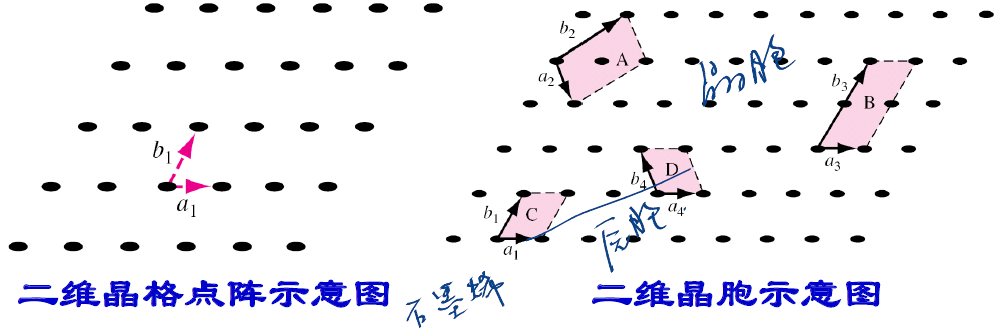
\includegraphics[width = .8\linewidth ]{chapter1/lattice.png}
  \caption{二维晶胞和晶格}
  \label{fig-lattice}
\end{figure}
\begin{figure}[hbt]
  \centering
  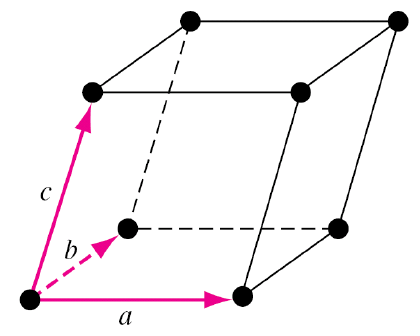
\includegraphics[width = .4\linewidth ]{chapter1/vector.png}
  \caption{晶胞基矢示意图}
  \label{fig-vector}
\end{figure}

常见的三个基本立方结构分别是\textbf{简单立方(SC,Simple Cubic)}、\textbf{体心立方(BCC,Body-Centered Cubic)}、\textbf{面心立方(FCC,Face-Centered Cubic)}。
立方体的边长即为\textbf{晶格常数}。

\subsection{晶向、晶面和密勒指数}
设$\vec{a}、\vec{b}、\vec{c}$是晶体的三个独立基矢,则连接任意两个格点的矢量可表示为:
\[ \vec{r} = l\vec{a} + m\vec{b} + n\vec{c}\]
取与\textit{l、m、n}成比例的三个互质整数\textit{u、v、w},并将他们放在方括号内,即[\textit{u v w}],用来表示特定的\textbf{晶向}。由晶体中的原子排列所构成的平面称为\textbf{晶面}。

设某晶面与$\vec{a}、\vec{b}、\vec{c}$轴的截距分别是\textit{p、q、s},且\textit{p、q、s}为整数\footnote{原点是任意的},取与\textit{p、q、s}各自的倒数成比例的三个互质的整数\textit{h、k、l},即
\[h: k: l=\frac{1}{p}: \frac{1}{q}: \frac{1}{s}\]
将它们放在圆括号内,即(\textit{h、k、l}),用来表示特定晶面的取向。这组晶面指数就是密勒指数。如图\ref{fig-index}为几个特定的晶向和晶面示意图。
\begin{figure}[hbt]
  \centering
  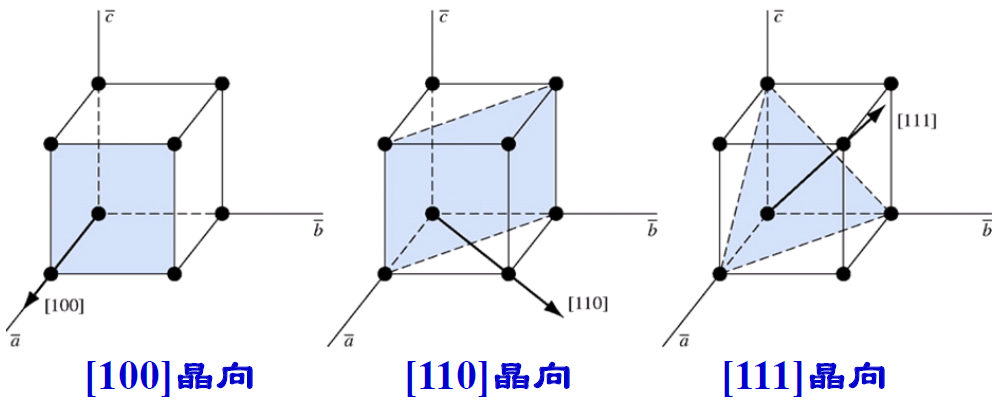
\includegraphics[width = .8\linewidth ]{chapter1/orientation.png}
  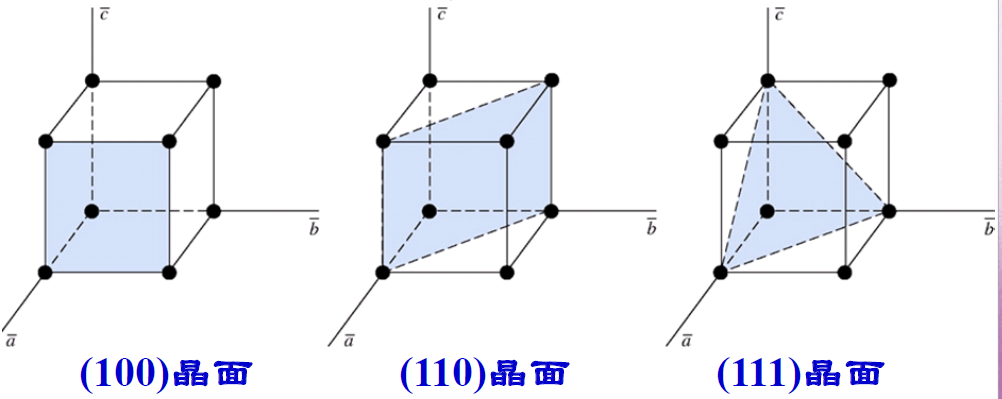
\includegraphics[width = .8\linewidth ]{chapter1/millerindex.png}
  \caption{晶向指数和晶面指数}
  \label{fig-index}
\end{figure}

\subsection{金刚石结构}
硅、锗等半导体材料都是金刚石结构,如图所示。Si的晶格常数为5.43\AA,Ge的晶格常数为5.65\AA。

\section{量子力学基础}

\section{能带模型}